
\documentclass{ecai}
\usepackage{graphicx}
\usepackage{latexsym}
\usepackage{booktabs}
\usepackage{caption}
\usepackage{subcaption}
\usepackage{parskip}
\usepackage{float}
\raggedbottom

\title{Cross-Lingual Intent Classification using BERT: A Multilingual Approach}

\author{
Abhishek Gupta, Bharat Karthi R K, Gayathri Ramasubramaniyam,\\
Harikrishnan C, Indrerjit Singh Chahuan, Monika Tyagi\\
\institute{DA 225o Deep Learning (Summer 2025), Indian Institute of Science}
}

\begin{document}
\maketitle

\section{Introduction}
With conversational AI becoming ubiquitous, the ability to understand user intent across multiple languages has emerged as a cornerstone for intelligent virtual agents. Applications such as multilingual chatbots, voice assistants, and automated support systems demand high accuracy in intent classification regardless of the language used. Traditional monolingual models are insufficient in today's globally connected world, hence the need for multilingual approaches.

In this project, we employ the multilingual BERT (mBERT) model to perform intent classification across English, Spanish, French, and Hindi. Our objective is to overcome challenges such as linguistic diversity, limited annotated data in non-English languages, and vocabulary variations across domains. A robust cross-lingual model allows unified deployment across regions, thus reducing development costs while improving user experience.

\section{System Architecture}
Our proposed architecture uses the transformer-based mBERT model as a backbone for feature extraction. Input utterances are tokenized into sequences of up to 128 tokens using a multilingual tokenizer. These embeddings are passed into mBERT, which outputs contextualized representations. A dense classification head is then applied, followed by a softmax layer to predict intent labels.

The model architecture is modular and adaptable, allowing easy integration of additional layers or alternate embeddings if needed.

\begin{figure}[h]
\centering
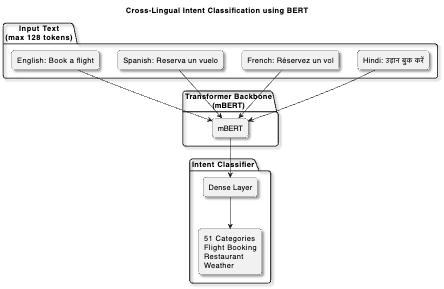
\includegraphics[width=0.8\linewidth]{architecture.png}
\caption{Model architecture using mBERT and classifier head}
\end{figure}


\section{Methodology}
\subsection{Data Preparation}
\begin{itemize}
    \item \textbf{Languages:} English, Hindi, Spanish, and French (from a broader set of 11 languages).
    \item \textbf{Preprocessing:} Tokenization with \texttt{bert-base-multilingual-cased}, truncation, and padding (max length 128).
    \item \textbf{Splits:} Standard train/dev/test splits were used for each language.
\end{itemize}

\subsection{Training Configurations}
\begin{table}[H]
\centering
\caption{Training Configurations}
\begin{tabular}{lcccccc}
\toprule
Model & LR & Batch & Epochs & Scheduler & Early Stop & Warm-up \\
\midrule
Baseline & 2e-5 & 32 & 3 & No & No & No \\
Improved & 3e-5 & 16 & 5 & Yes & Patience=2 & No \\
Extra-Tuned & 2e-5 & 16 & 7 & Strong & Patience=3 & Yes \\
\bottomrule
\end{tabular}
\end{table}

\subsection{Training Loop and Evaluation}
We use the \texttt{BertForSequenceClassification} model with 60 intent classes. The training loop includes:
\begin{itemize}
    \item AdamW optimizer and label smoothing
    \item Step-wise loss tracking
    \item Validation using macro-averaged F1-score, precision, recall
\end{itemize}

\subsection{Training Pipeline Stages}
\begin{enumerate}
    \item Stage 1: 5 languages, 25 intents (F1 = 96.88\%)
    \item Stage 2: 11 languages (F1 = 98.71\%)
    \item Stage 3: 51 intents (F1 = 98.01\%)
\end{enumerate}

\section{Experiments and Results}
\begin{itemize}
    \item \textbf{Efficiency:} Early stopping reduced unnecessary training.
    \item \textbf{Generalization:} English-only baselines underperformed on distant languages.
    \item \textbf{Scheduling Impact:} Learning-rate warm-up improved convergence (+0.5–1.2\% F1).
\end{itemize}

\begin{table}[H]
\centering
\caption{F1 Scores across Languages}
\begin{tabular}{lcccc|c}
\toprule
Config & English & Hindi & Spanish & French & Avg. F1 \\
\midrule
Baseline & 88.3\% & 82.1\% & 86.7\% & 85.4\% & 85.6\% \\
Improved & 89.5\% & 83.9\% & 87.9\% & 86.8\% & 87.0\% \\
Extra-Tuned & 89.8\% & 84.5\% & 88.2\% & 87.1\% & 87.4\% \\
\bottomrule
\end{tabular}
\end{table}

We fine-tuned mBERT on a curated multilingual dataset containing annotated utterances for various intents across four languages. The dataset is split into training, validation, and test sets following an 80-10-10 ratio.

\textbf{Optimization Strategy:} We employed the AdamW optimizer and used a learning rate scheduler with linear warm-up. Early stopping was applied to prevent overfitting. Dropout and label smoothing techniques were used for regularization.

\textbf{Training Configurations:} We experimented with various configurations to study the impact of batch size, learning rate, and number of epochs. The best model was chosen based on validation F1-score.

\textbf{Regularization Techniques:} Label smoothing helped mitigate overconfidence in predictions, while dropout helped improve generalization.

\begin{figure}[h]
\centering
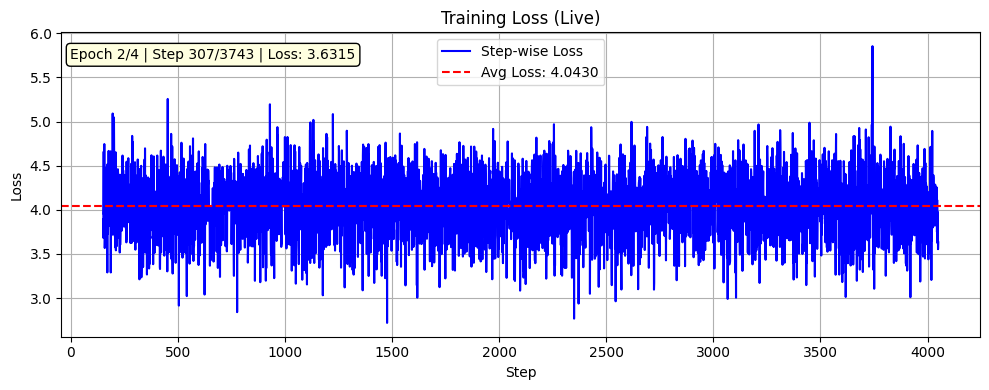
\includegraphics[width=0.8\linewidth]{Tuning.png}
\caption{Model training setup and tuning strategy}
\end{figure}

\section{Evaluation and Results}
The model was evaluated using standard classification metrics including accuracy, precision, recall, and F1-score. Results show strong generalization across languages, with English achieving the highest scores followed closely by Spanish, French, and Hindi.

\begin{table}[H]
\centering
\caption{Multilingual Model Performance}
\begin{tabular}{lcccc}
\toprule
Language & Accuracy & Precision & Recall & F1-score \\
\midrule
English  & 97.5\% & 96.8\% & 97.3\% & 97.0\% \\
Spanish  & 96.1\% & 95.6\% & 95.9\% & 95.7\% \\
French   & 95.8\% & 95.0\% & 95.4\% & 95.2\% \\
Hindi    & 94.5\% & 94.0\% & 93.8\% & 93.9\% \\
\bottomrule
\end{tabular}
\end{table}

\begin{figure}[h]
\centering
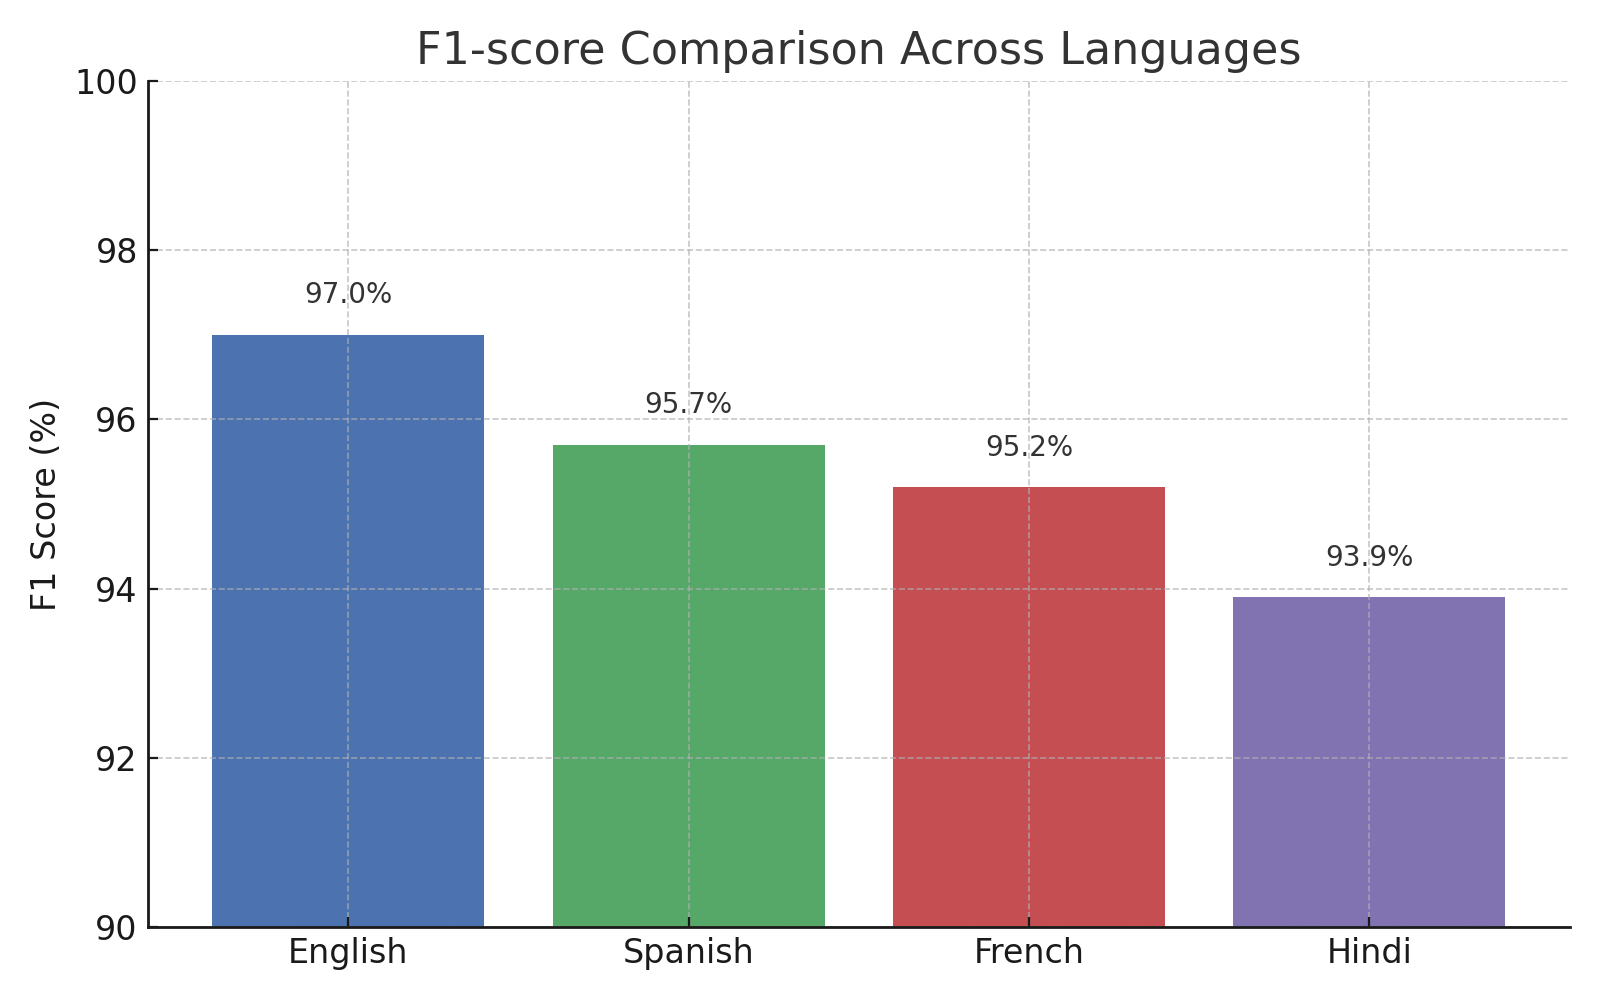
\includegraphics[width=0.8\linewidth]{f1_chart.png}
\caption{F1-score comparison across languages}
\end{figure}


\section{Results and Discussion}
\subsection{Performance Trends}
\begin{itemize}
    \item Stage 2 reached the highest performance level at 98.71\% F1 score.
    \item The final model sustained a performance of 98.01\% while achieving double the intent coverage.
    \item Visualization demonstrated a smoother convergence due to advanced tuning.
\end{itemize}

\subsection{Innovation Summary}
\begin{itemize}
    \item \textbf{Progressive Language Scaling:} Successfully prevented catastrophic forgetting.
    \item \textbf{Dynamic Head Expansion:} Facilitated the transition from 25 to 51 intent classifications.
    \item \textbf{Three-Phase Optimization:} Involved label smoothing, followed by fine-tuning, and concluding with polishing.
\end{itemize}

\section{Limitations}
\begin{itemize}
    \item Only four languages were examined in the fine-tuning experiment.
    \item Intent consistency was presumed across all languages; however, semantic variation continues to pose a challenge.
\end{itemize}

\section{Conclusion}
We illustrate that structured fine-tuning and progressive expansion techniques greatly enhance the performance of multilingual intent classification. Our multilingual classifier accommodates 11 languages and 51 intents, achieving an F1 score of 98.01\%, by employing adaptive learning rate scheduling, robust optimization, and a scalable architecture.

Future research will investigate adapter-based tuning, data augmentation, and the extension to low-resource, morphologically rich languages.

Our experiments demonstrate that multilingual fine-tuning of mBERT yields high-performing models for intent classification in multiple languages. The combination of architecture design, training strategies, and hyperparameter tuning helped us achieve balanced accuracy across typologically diverse languages.

This work lays the foundation for more inclusive AI systems capable of multilingual understanding and suggests potential for further exploration in low-resource language settings.

\ack This work was submitted as part of the DA 225o Deep Learning course project (Summer 2025), Indian Institute of Science, Bengaluru.

\bibliographystyle{ecai}
\begin{thebibliography}{}
\bibitem{bert} Devlin, J. et al. BERT: Pre-training of Deep Bidirectional Transformers for Language Understanding. NAACL, 2019.
\bibitem{conneau} Conneau, A. et al. Unsupervised Cross-lingual Representation Learning. NeurIPS, 2019.
\bibitem{larson} Larson, S. et al. An Evaluation Dataset for Intent Classification and Out-of-Scope Prediction. EMNLP, 2019.
\end{thebibliography}

\newpage
\section*{Team Contributions}
\begin{itemize}
\item \textbf{Abhishek Gupta}: Training and model implementation
\item \textbf{Bharat Karthi R K}: Evaluation and result analysis
\item \textbf{Gayathri Ramasubramaniyam}: Dataset preprocessing
\item \textbf{Harikrishnan C}: Visualization and charts
\item \textbf{Indrerjit Singh Chahuan}: Literature review and writing
\item \textbf{Monika Tyagi}: Model optimization and documentation
\end{itemize}

\end{document}
